\documentclass[fontsize=12pt,DIV=11,BCOR=4mm,fleqn]{scrartcl}
\KOMAoptions{footnotes=multiple}

\usepackage[hyphens]{url}
\usepackage[
	bookmarksopen,
	colorlinks=false,
	linktoc=all,
	linkcolor=red,
	citecolor=green,
	urlcolor=blue,
	pdftitle={Systemnahe Programmierung}, 
	pdfauthor={Mehmet Ali Incekara, Tom Wolske, Heiko Faller}
]{hyperref}

\usepackage[margin=3cm]{geometry}

\usepackage{tocloft}
\renewcommand{\cftsecleader}{\cftdotfill{\cftdotsep}}

\usepackage[yyyymmdd]{datetime}
\renewcommand{\dateseparator}{.}

\usepackage{enumitem}
\setlist[description]{style=nextline}

\setkomafont{section}{\Huge} 
\setkomafont{subsection}{\Large}

\usepackage[nonumberlist,acronym,toc,section]{glossaries}
\renewcommand*{\glspostdescription}{}
\makeglossaries
\include{acronym}
\include{glossar}
\glsaddall
\bibliographystyle{plaindin}

\usepackage[onehalfspacing]{setspace} 

\usepackage{fontspec}
\usepackage{microtype}
\usepackage{graphicx}
\usepackage[svgnames,table]{xcolor}
\usepackage{xcolor}
\usepackage{amsmath}
\usepackage{multicol}
\usepackage[ngerman]{babel}
\usepackage[babel,german=quotes]{csquotes}
\usepackage{eurosym}

\usepackage{listings}
\setlist[description]{style=nextline}
\definecolor{light-gray}{gray}{0.95}
\definecolor{mygreen}{rgb}{0,0.6,0}

\newcommand{\minitab}[2][c]{\begin{tabular}{#1}#2\end{tabular}}
\newcolumntype{/}{>{\global\let\currentrowstyle\relax}}
\newcolumntype{^}{>{\currentrowstyle}}
\newcommand{\rowstyle}[1]{\gdef\currentrowstyle{#1}%
  #1\ignorespaces
}

\usepackage{scrlayer-scrpage}
\automark{subsection}

\clearscrheadings
\setlength{\footheight}{36pt}
\setlength{\headheight}{28pt}
\ohead{\rightmark}
\cfoot{\\Seite \pagemark}
\pagestyle{scrheadings}

\renewcommand{\contentsname}{Inhaltsverzeichnis}
\renewcommand{\listfigurename}{Abbildungsverzeichnis}
\renewcommand{\figurename}{Abbildung}
\renewcommand{\listtablename}{Tabellenverzeichnis}
\renewcommand{\tablename}{Tabelle}

\setlength{\parindent}{0pt}

\begin{document}
	\begin{titlepage}
		\fontspec{Times New Roman}
		\begin{center}
			
\includegraphics[width=8cm]{dhbw.pdf}
			
			\vfill
			\begin{singlespacing}
				{\Huge TITEL UND SO} \vspace{1.7cm}
				{\Large JSADOKAS}	\\ [0.25cm]
				{\large des Studiengangs Angewandte Informatik}	\\ [0.25cm]
				{\large an der Dualen Hochschule Baden-Württemberg Karlsruhe}	\\[0.25cm]
				{\large von} 	\\ [0.25cm]
				{\large \bfseries Heiko Faller, Mehmet Ali Incekara und Tom Wolske}	\\ [1cm]
			\end{singlespacing} 
			\vfill
		\end{center}
	\end{titlepage}
	\clearscrheadings
	
	\vspace*{2.5cm}
	\section*{Ehrenwörtliche Erklärung}
	gemäß § 5 (3) der "`Studien- und Prüfungsordnung DHBW Technik"' vom 22. September 2011. \vspace{5pt}

	Ich habe die vorliegende Arbeit mit dem Titel
	
	\begin{center}
		"` TITEL "'
	\end{center}
	
	selbstständig verfasst und keine anderen als die angegebenen Quellen und Hilfsmittel verwendet.

	\vspace{2cm}
	\makebox[7cm][l]{Montabaur, den \the\day.\the\month.\the\year}	\hfill	\\ %\makebox[5cm][c]{
\includegraphics{Unterschrift_ali.png}} \\
	\rule{5cm}{0.4pt} \hfill	\rule{5cm}{0.4pt} \\
	\makebox[7cm][l]{Ort, Datum} \hfill	\makebox[5cm][c]{Mehmet Ali Incekara} 
	
	\pagebreak{}
	\clearpage
	\vspace*{2.1cm}
	\section*{Sperrvermerk}
		Die vorliegende Praxisarbeit mit dem Titel 
		
		\begin{center}
			"` TITEL "'
		\end{center}
		
		enthält vertrauliche Daten des Unternehmens 1\&1 Internet SE. \vspace{5pt}
	
		Diese Praxisarbeit darf nur vom Gutachter sowie berechtigten des Prüfungsausschusses eingesehen werden. Eine Vervielfältigung und Veröffentlichung der Praxisarbeit ist auch auszugsweise nicht erlaubt. \vspace{5pt}
	
		Dritten darf diese Arbeit nur mit der ausdrücklichen Genehmigung des Verfassers und Unternehmens zugänglich gemacht werden.
	
	\pagebreak{}
	\clearpage
	\vspace*{0.1cm}
	\tableofcontents{} \thispagestyle{empty} \addtocontents{toc}{\par}
	\addtocontents{toc}{\protect\thispagestyle{empty}}
	
	\pagebreak{}
	\clearpage
	\clearscrheadings
	\pagenumbering{Roman}
	\cfoot{\pagemark}
	\setcounter{page}{5} 
	\vspace*{2.5cm}
	\listoffigures{}\addtocontents{lof}{\par}
	\addcontentsline{toc}{section}{Abbildungsverzeichnis}
	
	\pagebreak{}
	\vspace*{2.5cm}
	\listoftables{}\addtocontents{lot}{\par}
	\addcontentsline{toc}{section}{Tabellenverzeichnis} 
	
	\pagebreak{}
	\clearscrheadings
	\pagenumbering{arabic}
	\cfoot{\pagemark}
	\setcounter{page}{1} 
	
	\section{Einleitung}
		einasd
		\pagebreak{}
	\section{Grundlagen}
		\subsection{Der Mikrocontroller}
	Ein Mikrocontroller ist ein Ein-Chip-Computersystem, der einen Prozessor und Peripheriefunktionen beinhaltet. In den meisten Fällen befindet sich der Arbeits- und Programmspeicher teilweise oder auch komplett auf demselben Chip. 
	
	In der Industrie ist der Mikrocontroller bereits seit vielen Jahren ein nicht mehr wegzudenkendes Bauteil. Sie werden im Alltag in eingebetteten Systemen verwendet, zum Beispiel in Waschmaschinen, Fernsehgeräte und sogar im Fahrzeug als Steuergeräte für das Antiblockiersystem (ABS), Airbag usw.
	
	Mikrocontroller können in verschienden Sprachen programmiert werden. Welche sich jedoch am besten eignet, ist vom Anwendungsfall abhängig. Assembler eignet sich besonders, da es einen direkten Einstieg in die Hardware bietet und keine Abhängigkeiten zu anderen Compilern hat.\footnote{http://www.mikrocontroller.net/articles/AVR-Tutorial}. 
	
\subsection{Assembler}
	Ein Assembler ist ein Übersetzer für Programmcode, der sich aus Maschinenbefehlen zusammensetzt. In der Art der verwendeten Befehle besteht der wesentliche Unterschied zu allen anderen Programmiersprachen. 
	
	Während sich Befehle bei den Hochsprachen, wie beispielsweise Java und C++, in der Übersetzung aus mehreren Anweisungen im endgültigen Code zusammensetzen, wird der Assemblerbefehl durch den Assembler lediglich in die entsprechende Binärform übersetzt. Weiterhin ersetzt der Assembler Variablen durch die entsprechenden Speicheradressen\footnote{Vgl. http://assembler.hpfsc.de/}.
	
\subsection{MSC-8051}
	Der MSC-8051 ist die Bezeichnung einer von Intel vorgestellten Familie von 8-Bit-Mikrocontrollern.
	
	
	% \footnote{http://www.mikrocontroller.net/articles/8051}
	
	% \footnote{https://de.wikipedia.org/wiki/Intel_MCS-51}

\subsection{MCU 8051 IDE}
	Die MCU 8051 IDE ist eine grafische Entwicklungsumgebung für Mikrocontroller, die auf dem MSC-8051 basieren. Das folgende Bild stammt von der Homepage\footnote{http://www.moravia-microsystems.com/mcu-8051-ide/} der Entwicklungsumgebung. Es zeigt im Hintergrund den Aufbau der IDE und im Vordergrund einige Simulationsfeatures. 

	\begin{center}
		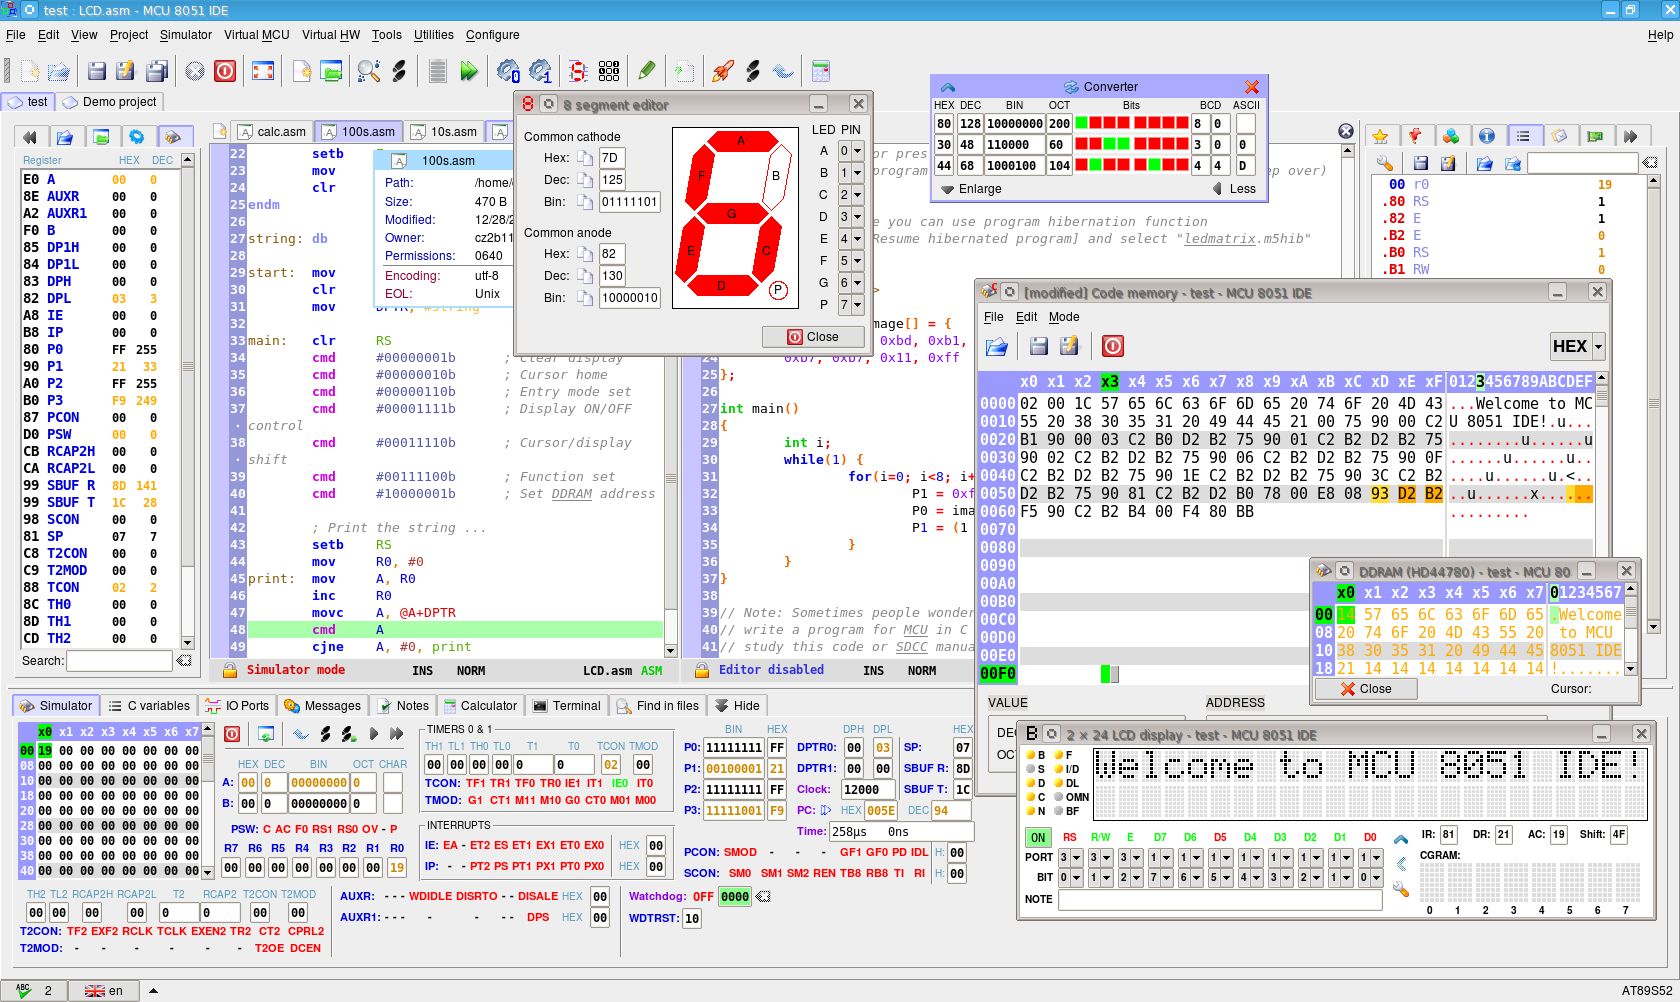
\includegraphics[width=\textwidth]{mcu8051ide.png}
		\captionof{figure}[MCU 8051 IDE]{MCU 8051 IDE} 
	\end{center}
	
	Die Simulation ist eine Softwarekomponente zur Simulation des Mikrocontrollers in einer virtuellen Umgebung. Zusätzliche Features erweitern die Möglichkeit den Mikrocontroller zu simulieren. Beispielsweise gibt es Hardware-Komponenten wie Schalter, Timer und Temperatur Sensor.
		\pagebreak{}
	\section{Konzept}
		\subsection{Konzept und Idee}

Die Idee ist es, ein SmartHome zu entwickeln, welches auf einem 8051 Microcontroller als Grundlage aufbaut. Dabei sollen drei Hauptfunktionen eines modernen SmartHomes über diesen gesteuert werden.

Die erste Funktion ist eine Temperatursteuerung für die Fußbodenheizung. Dabei soll die Fußbodenheizung in einem Haus so gesteuert werden, dass diese automatisch eingeschaltet wird, sobald die Temperatur unter einen festen Wert fällt. Außerdem soll der Nutzer mit Hilfe eines Schalters festlegen können, ob die Heizung dauerhaft an oder in einen automatischen Modus eingestellt ist. Der Temperatursensor ist zusätzlich abschaltbar, damit die Heizung ausgeschaltet werden kann.

Wird der Heizungsschalter auf An gestellt, läuft die Heizung unabhängig von der Temperatur die ganze Zeit. Wird dieser auf den Automodus gestellt, kommt es auf den Temperatursensor an, da dieser unabhängig von der Heizung ein bzw. ausgeschaltet werden kann. Ist dieser eingeschaltet, schaltet sich die Heizung an, sobald die Temperatur unter einen bestimmten Wert fällt.
Aus diesen Anforderungen ergibt sich eine Tabelle aus der alle möglichen Eingaben und Ausgabemöglichkeiten ausgelesen werden können. Aus diesen geht ein Schaltplan hervor, welcher für die Programmierung des 8051 Microcontrollers genutzt wird.
Die Tabelle sieht wie folgt aus:

\begin{table}[htbp]
\centering
\caption{Schaltplan Heizungssteuerung}
\label{my-label}
\begin{tabular}{|l|l|l|l|}
\hline
\multicolumn{1}{|c|}{\textbf{Heizungsschalter}} & \multicolumn{1}{c|}{\textbf{Temperatursensor Schalter}} & \multicolumn{1}{c|}{\textbf{Temperatur < Wert}} & \multicolumn{1}{c|}{\textbf{Heizung An?}} \\ \hline
 0 & 0 & 0 & 0 \\ \hline
 0 & 0 & 1 & 0 \\ \hline
 0 & 1 & 0 & 0 \\ \hline
 0 & 1 & 1 & 1 \\ \hline
 1 & 0 & 0 & 1 \\ \hline
 1 & 0 & 1 & 1 \\ \hline
 1 & 1 & 0 & 1 \\ \hline
 1 & 1 & 1 & 1 \\ \hline
\end{tabular}
\end{table}

Für diese Steuerung wird die Schaltung nach diesem Schaltplan programmiert:

\begin{figure}[htbp] 
  \centering
     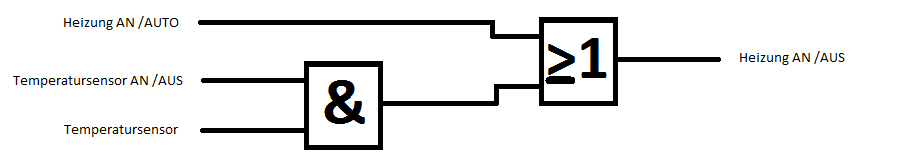
\includegraphics[width=0.7\textwidth]{Heizungsschaltung.png}
  \caption{Schaltung für die Heizung}
  \label{fig:Bild1}
\end{figure}

Dabei kommen die Eingaben aus dem Port 2.0 bis 2.2 und die Ausgabe ist auf dem Port 3.4.
Die zweite Funktion ist eine Lichtsteuerung für das Licht. Der Nutzer soll die Möglichkeit haben das Licht mit Hilfe eines Bewegungssensors ein beziehungsweise aus zu schalten. Dieser Sensor ist zusätzlich an einen Schalter angeschlossen, um diesen An bzw. Aus zu schalten.
 
Aus diesen Anforderungen ergibt sich eine Tabelle aus der alle möglichen Eingaben und Ausgabemöglichkeiten ausgelesen werden können. Aus diesen geht ein Schaltplan hervor, welcher für die Programmierung des 8051 genutzt wird.

\begin{table}[htbp]
\centering
\caption{Schaltplan Lichtsteuerung}
\label{my-label}
\begin{tabular}{|l|l|l|}
\hline
\multicolumn{1}{|c|}{\textbf{Bewegungssensor}} & \multicolumn{1}{c|}{\textbf{Schalter}} & \multicolumn{1}{c|}{\textbf{Licht an?}} \\ \hline
 0 & 0 & 0 \\ \hline
 0 & 1 & 0 \\ \hline
 1 & 0 & 0 \\ \hline
 1 & 1 & 1 \\ \hline
\end{tabular}
\end{table}

Für diese Steuerung wird die Schaltung nach diesem Schaltplan programmiert:

\begin{figure}[htbp] 
  \centering
     
\includegraphics[width=0.7\textwidth]{Lichtschaltung.png}
  \caption{Schaltung für das Licht}
  \label{fig:Bild2}
\end{figure}

Dabei kommen die Eingaben aus den Ports P1.0 und 1.1 und die Ausgabe ist auf dem Port 3.5.
Der dritte Teil der SmartHome Steuerung ist eine Steuerung für Rollläden. Diese sollen automatisch aufgehen, sobald es draußen hell, beziehungsweise zu gehen, sobald es draußen dunkel wird. Dabei gehen diese komplett auf und zu. Dafür werden kontakte an der Ober- und Unterseite der Rollläden genutzt. Für die automatische Steuerung wird ein Helligkeitssensor genutzt.
Aus diesen Anforderungen geht wie zuvor auch eine Tabelle hervor:

\begin{table}[]
\centering
\caption{Rolladensteuerung manuell}
\label{my-label}
\begin{tabular}{|l|l|l|l|l|l|}
\hline
\multicolumn{1}{|c|}{\textbf{SR Oben}} & \multicolumn{1}{c|}{\textbf{SR Unten}} & \multicolumn{1}{c|}{\textbf{SR Hoch}} & \multicolumn{1}{c|}{\textbf{SR Runter}} & \multicolumn{1}{c|}{\textbf{MR Hoch}} & \multicolumn{1}{c|}{\textbf{MR Runter}} \\ \hline
 0 & 0 & 0 & 0 & 0 & 0 \\ \hline
 0 & 0 & 0 & 1 & 0 & 1 \\ \hline
 0 & 0 & 1 & 0 & 1 & 0 \\ \hline
 0 & 0 & 1 & 1 & 0 & 0 \\ \hline
 0 & 1 & 0 & 0 & 0 & 0 \\ \hline
 0 & 1 & 0 & 1 & 0 & 0 \\ \hline
 0 & 1 & 1 & 0 & 1 & 0 \\ \hline
 0 & 1 & 1 & 1 & 0 & 0 \\ \hline
 1 & 0 & 0 & 0 & 0 & 0 \\ \hline
 1 & 0 & 0 & 1 & 0 & 1 \\ \hline
 1 & 0 & 1 & 0 & 0 & 0 \\ \hline
 1 & 0 & 1 & 1 & 0 & 0 \\ \hline
 1 & 1 & 0 & 0 & 0 & 0 \\ \hline
 1 & 1 & 0 & 1 & 0 & 0 \\ \hline
 1 & 1 & 1 & 0 & 0 & 0 \\ \hline
 1 & 1 & 1 & 1 & 0 & 0 \\ \hline
\end{tabular}
\end{table}


\begin{table}[]
\centering
\caption{Rolladensteuerung automatisch}
\label{my-label}
\begin{tabular}{|l|l|l|l|l|}
\hline
\multicolumn{1}{|c|}{\textbf{SR Oben}} & \multicolumn{1}{c|}{\textbf{SR Unten}} & \multicolumn{1}{c|}{\textbf{Helligkeitssensor}} & \multicolumn{1}{c|}{\textbf{MR Hoch}} & \multicolumn{1}{c|}{\textbf{MR Runter}} \\ \hline
0 & 0 & 0 & 0 & 1 \\ \hline
0 & 0 & 1 & 1 & 0 \\ \hline
0 & 1 & 0 & 0 & 0 \\ \hline
0 & 1 & 1 & 1 & 0 \\ \hline
1 & 0 & 0 & 0 & 1 \\ \hline
1 & 0 & 1 & 0 & 0 \\ \hline
1 & 1 & 0 & 0 & 0 \\ \hline
1 & 1 & 1 & 0 & 0 \\ \hline
\end{tabular}
\end{table}

		\pagebreak{}
	\section{Umsetzung}
		\subsection{Rolladen-Steuerung}
	Die Schwierigkeit bei der Entwicklung der Rollladenschaltung war, dass eine Menge Port-Bits benötigt werden, weshalb wir uns dazu entschieden haben, ein Modell zur Steuerung von zwei Rollläden zu wählen. Als erstes wird das Automodus-Bit abgefragt, um zu entscheiden, ob der Automodus eingesetzt wird oder die Röllläden manuell gesteuert werden.
\subsubsection{Manuelle Steuerung}
Im manuellen Modus wird bei den Röllläden abwechselnd überprüft, ob sie hoch oder runter fahren sollen. Dazu wird mittels Polling jeweils abgefragt, wie die Schalterpositionen sind und ob der zu überprüfende Rollladen oben oder unten ist. Dementsprechend werden dann die Motoren angesteuert. Es werden dabei immer die Zustände beider Schalter, also sowohl für hoch als auch für runter, abgefragt. Das dient dazu, den fehlerhaften Zustand, dass beide aktiviert sind zu umgehen. In diesem Fall würde der Rollladen dann einfach nicht starten, als wären beide Schalter inaktiv. \\
Die Abfragen laufen folgendermaßen ab:
Zuerst wird bei beiden Rollläden nach folgendem Schema geprüft, ob sie nach oben fahren sollen.
\begin{enumerate}
\item{Rolladen nicht oben?}
\item{Schalter hoch aktiviert?}
\item{Schalter runter deaktiviert?}
\item{Rolladen abhängig davon hochfahren}
\end{enumerate}
Daraufhin folgen, wieder für beide Rollläden, die Abfragen, um zu prüfen ob sie nach unten fahren müssen.
\begin{enumerate}
\item{Rolladen nicht unten?}
\item{Schalter runter aktiviert?}
\item{Schalter hoch deaktiviert?}
\item{Rolladen abhängig davon heruntergefahren}
\end{enumerate}

\subsubsection{Automodus}
Ist der automatische Modus aktiviert, ist die Position der Schalter egal, da diese nicht mehr abgerufen werden. Stattdessen kommt ein Helligkeitssensor zum Einsatz, der bei anschlägt, wenn es draußen hell ist. In diesem Fall werden also das Sensor-Bit, sowie wieder die Positionssensoren, abgefragt.
Zuerst kommt wieder für beide Rollläden die Prüfung, ob er nach oben fahren soll.

\begin{enumerate}
\item{Rolladen nicht oben?}
\item{Helligkeitssensor schlägt an?}
\item{Rolladen abhängig davon hochfahren}
\end{enumerate}
Abschließend kommen nun noch die Abfragen, ob die Rollläden nach  unten fahren sollen.
\begin{enumerate}
\item{Rolladen nicht unten?}
\item{Helligkeitssensor schlägt nicht an?}
\item{Rolladen abhängig davon heruntergefahren}
\end{enumerate}


\subsection{Licht-Steuerung}
	Bei der Lichtsteuerung werden einfach die Eingänge verundet und das Ergebnis an das Licht ausgegeben. Der Ablauf sieht also folgendermaßen aus.
\enuerate{begin}
\item{Automatische Lichtsteuerung aktiviert?}
\item{Sensor schlägt an?}
\item{Licht davon abhängig an- beziehungsweise ausschalten}
\enumerate{end}


\subsection{Heizung-Steuerung}
	Ein Temperatursensor liefert der Heizungssteuerung die Information, ob die Temperatur sich unter dem Fixwert befindet. Wenn das der Fall ist und die automatische Steuerung aktiv ist wird die Heizung aktiv. Unabhängig davon wird die Heizung auch aktiv, wenn dier Schalter betätigt wird. Daraus ergibt sich folgender Ablauf:

\begin{enumerate}
	\item {Sensor schlägt an?}
	\item {Automatische Steuerung aktiviert?}
	\item {oder manuelle Steuerung aktiviert?}
	\item {Heizung davon abhängig an- beziehungsweise ausschalten}
\end{enumerate}

		\pagebreak{}
	\section{Zusammenfassung}
		Ziel war die beispielhafte Entwicklung einer Smarthome Haussteuerung auf dem Mikrocontroller 8051. Dabei wurden drei verschiedene Funktionen umgesetzt:

\begin{itemize}
	\item {Eine Heizungssteuerung}
	\item {Eine Lichtsteuerung}
	\item {Eine Rolladensteueung}
\end{itemize}

Diese Funktionen wurden in dem Emulator MCU 8051 programmiert und beispielhaft ausgeführt.


Abschließend kann gesagt werden, dass diese Funktionen funktionsfähig sind, der Funktionsumfang jedoch noch durch weitere nützliche Automatisierungen ergänzt werden kann. Dazu wird jedoch weitere Hardware benötigt und die Anzahl der Ports am 8051 Mikrokontroller sind begrenzt.


		
\end{document}